\documentclass[11pt]{article}

% ---- Packages ----------------------------------------------------------
\usepackage[margin=1in]{geometry}
\usepackage{graphicx}
\usepackage{subcaption}
\usepackage{float}
\usepackage{amsmath}
\usepackage[hidelinks]{hyperref}

% ---- Where to find the images ------------------------------------------
% Compile this file from inside the `figs/` directory.
\graphicspath{{N5/}{N6/}}

% ---- Title -------------------------------------------------------------
\title{Soliton Spin-Chain Heatmaps:\\ Real Space and Momentum--Energy ($k$--$\omega$) Space}
\author{Heisenberg Spin Chain --- Solitons}
\date{\today}

\begin{document}
\maketitle
\tableofcontents
\bigskip

\noindent For each parameter set we show the spin signal in real space
($\delta S$ over site $j$ and time $t$) alongside its two-dimensional
Fourier transform in momentum--energy space ($|S(k,\omega)|^2$). All runs use
a single initial condition (IC\,=\,1).

% =======================================================================
\section{$N = 5$ \quad ($L = 500$)}
% =======================================================================

\begin{figure}[H]
  \centering
  \begin{subfigure}{0.48\textwidth}
    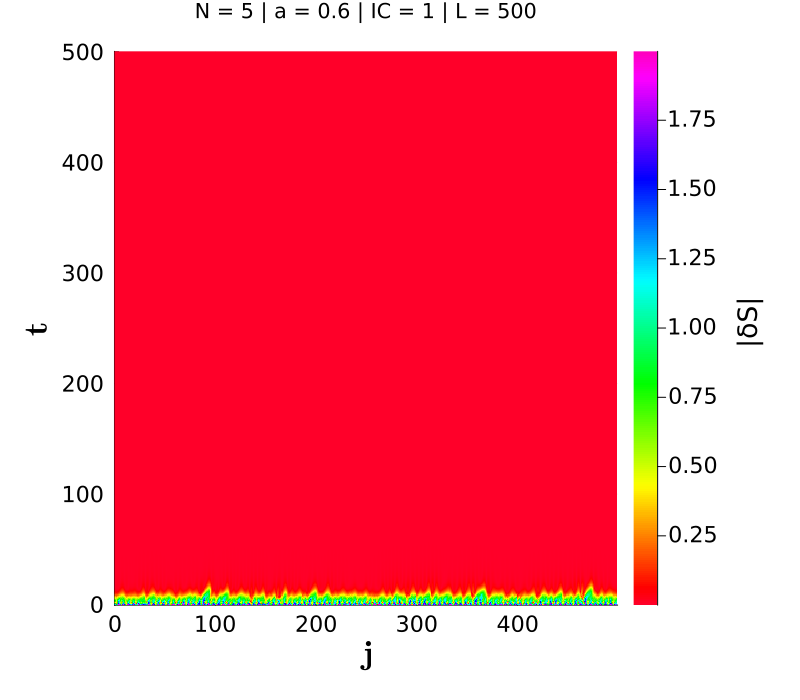
\includegraphics[width=\linewidth]{N5/a0p6_IC1_L500_trial1.png}
    \caption{Real space}
  \end{subfigure}\hfill
  \begin{subfigure}{0.48\textwidth}
    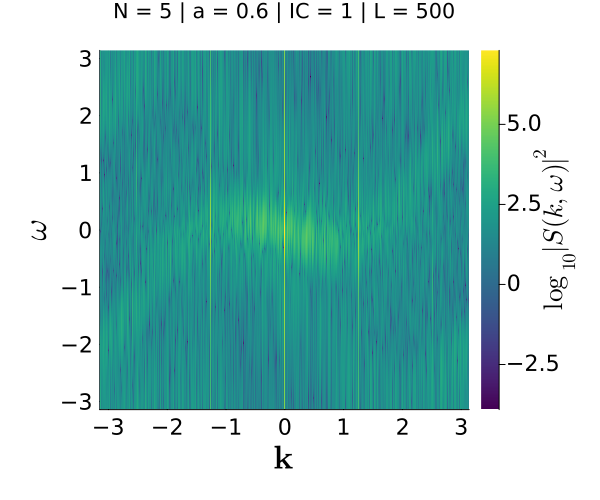
\includegraphics[width=\linewidth]{N5/a0p6_IC1_L500_trial1_komega.png}
    \caption{$k$--$\omega$ space}
  \end{subfigure}
  \caption{$N = 5$, $a = 0.6$, $L = 500$.}
\end{figure}

\begin{figure}[H]
  \centering
  \begin{subfigure}{0.48\textwidth}
    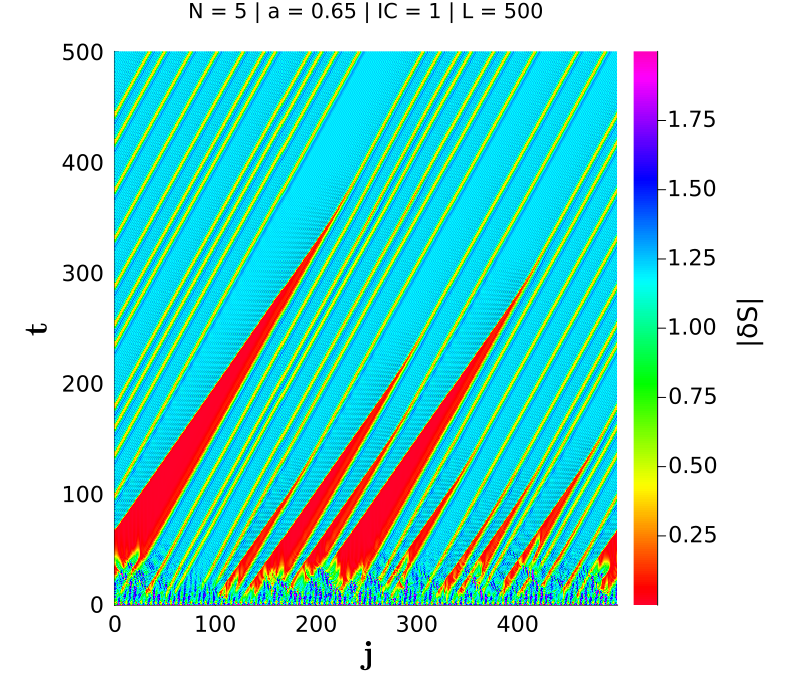
\includegraphics[width=\linewidth]{N5/a0p65_IC1_L500_trial1.png}
    \caption{Real space}
  \end{subfigure}\hfill
  \begin{subfigure}{0.48\textwidth}
    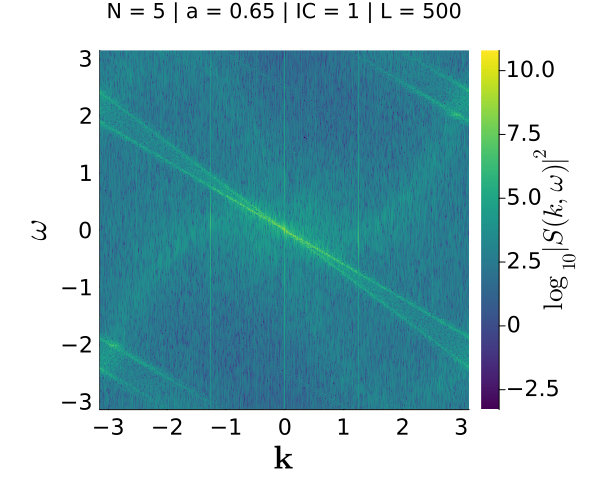
\includegraphics[width=\linewidth]{N5/a0p65_IC1_L500_trial1_komega.png}
    \caption{$k$--$\omega$ space}
  \end{subfigure}
  \caption{$N = 5$, $a = 0.65$, $L = 500$.}
\end{figure}

\begin{figure}[H]
  \centering
  \begin{subfigure}{0.48\textwidth}
    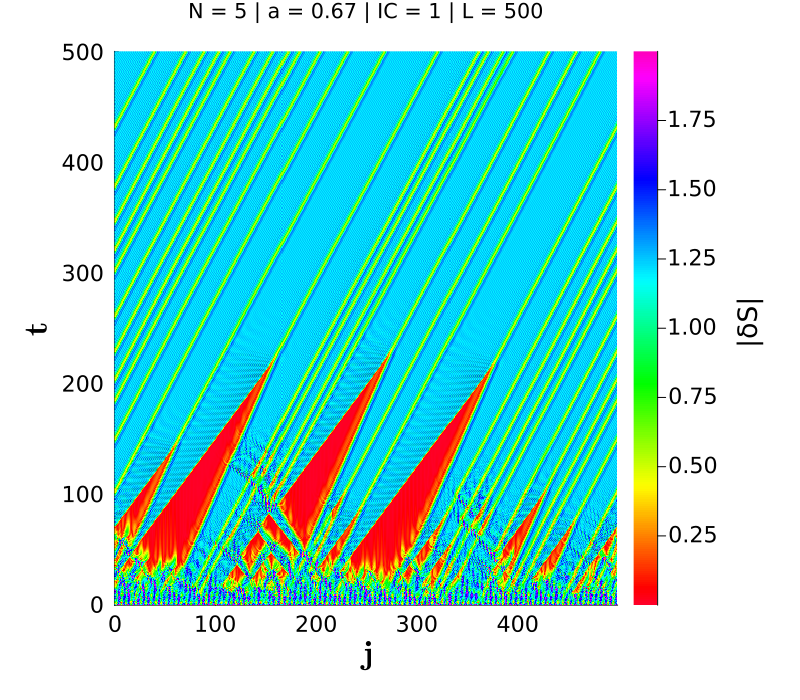
\includegraphics[width=\linewidth]{N5/a0p67_IC1_L500_trial1.png}
    \caption{Real space}
  \end{subfigure}\hfill
  \begin{subfigure}{0.48\textwidth}
    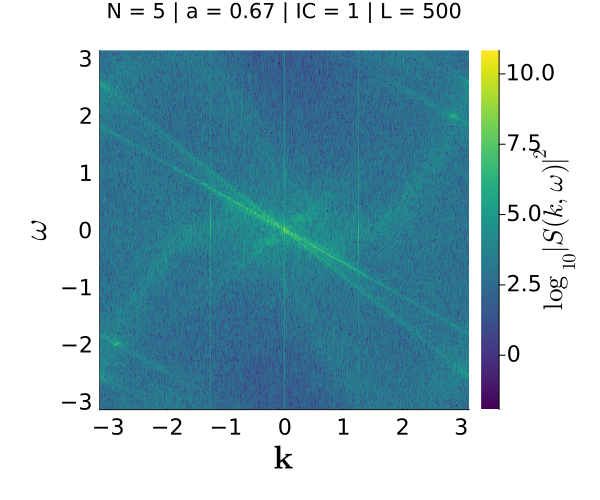
\includegraphics[width=\linewidth]{N5/a0p67_IC1_L500_trial1_komega.png}
    \caption{$k$--$\omega$ space}
  \end{subfigure}
  \caption{$N = 5$, $a = 0.67$, $L = 500$.}
\end{figure}

\begin{figure}[H]
  \centering
  \begin{subfigure}{0.48\textwidth}
    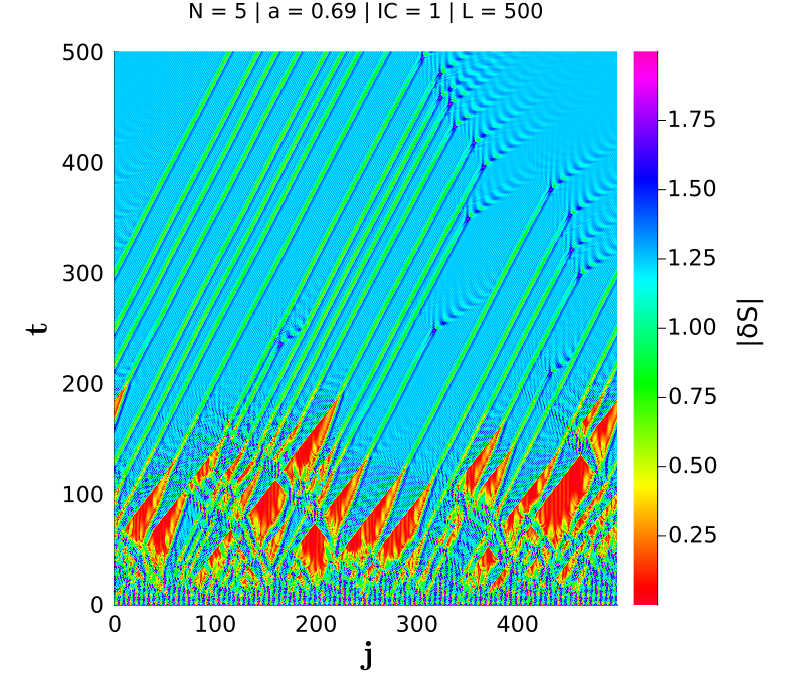
\includegraphics[width=\linewidth]{N5/a0p69_IC1_L500_trial1.png}
    \caption{Real space}
  \end{subfigure}\hfill
  \begin{subfigure}{0.48\textwidth}
    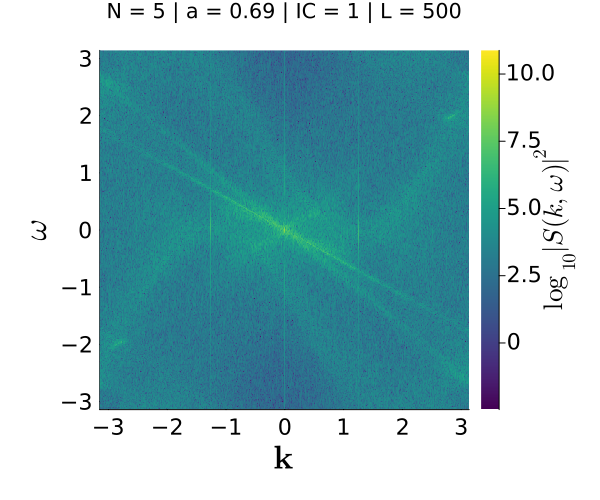
\includegraphics[width=\linewidth]{N5/a0p69_IC1_L500_trial1_komega.png}
    \caption{$k$--$\omega$ space}
  \end{subfigure}
  \caption{$N = 5$, $a = 0.69$, $L = 500$.}
\end{figure}

\begin{figure}[H]
  \centering
  \begin{subfigure}{0.48\textwidth}
    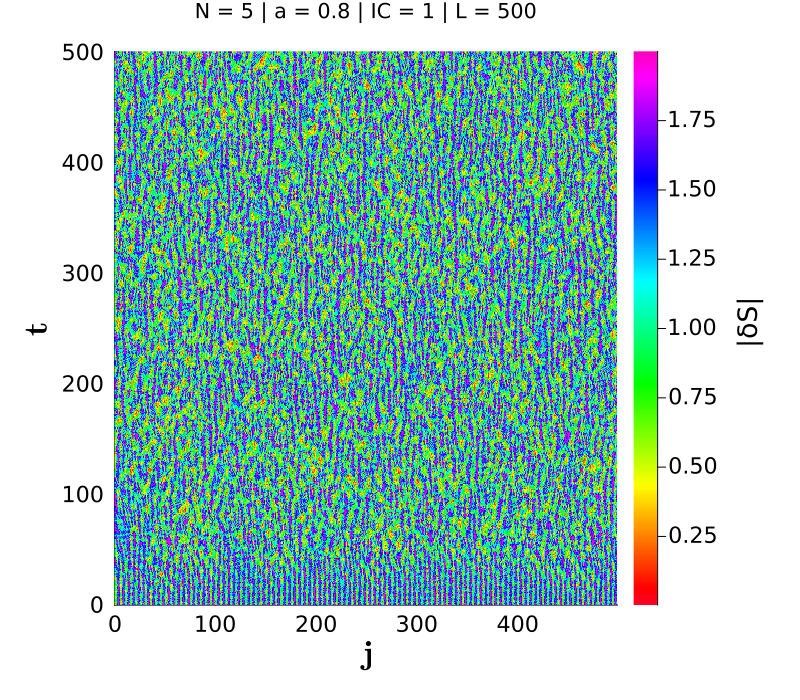
\includegraphics[width=\linewidth]{N5/a0p8_IC1_L500_trial1.png}
    \caption{Real space}
  \end{subfigure}\hfill
  \begin{subfigure}{0.48\textwidth}
    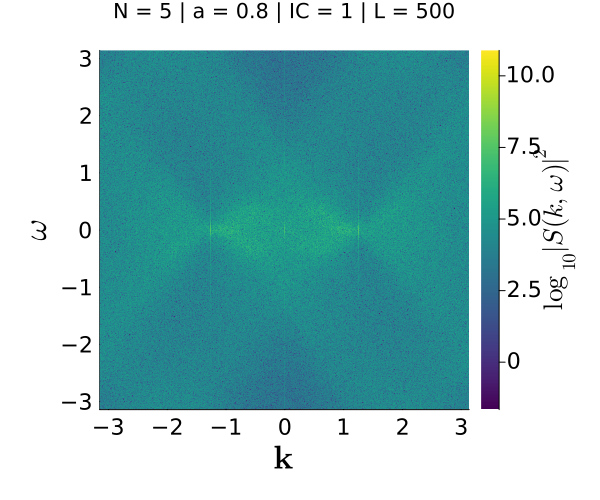
\includegraphics[width=\linewidth]{N5/a0p8_IC1_L500_trial1_komega.png}
    \caption{$k$--$\omega$ space}
  \end{subfigure}
  \caption{$N = 5$, $a = 0.8$, $L = 500$.}
\end{figure}

\begin{figure}[H]
  \centering
  \begin{subfigure}{0.48\textwidth}
    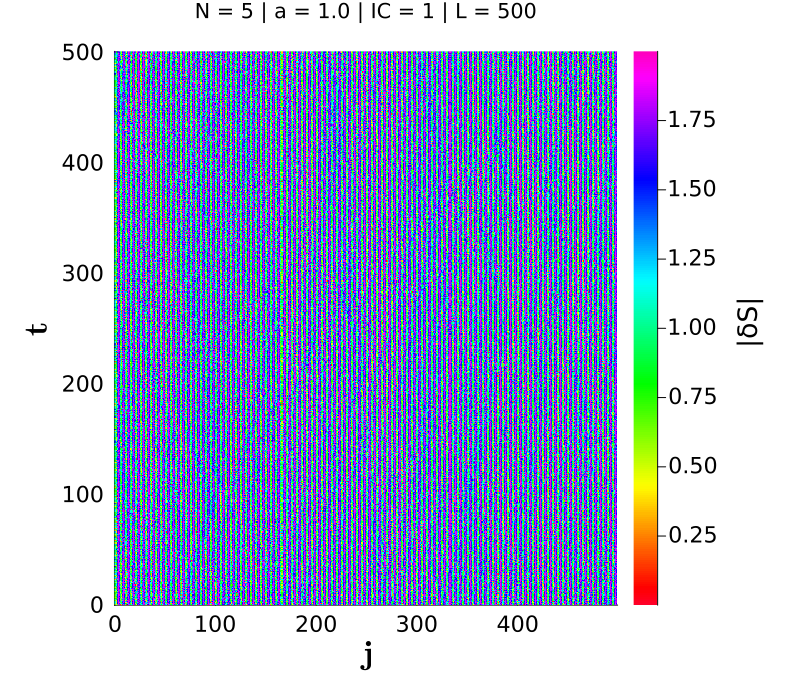
\includegraphics[width=\linewidth]{N5/a1p0_IC1_L500_trial1.png}
    \caption{Real space}
  \end{subfigure}\hfill
  \begin{subfigure}{0.48\textwidth}
    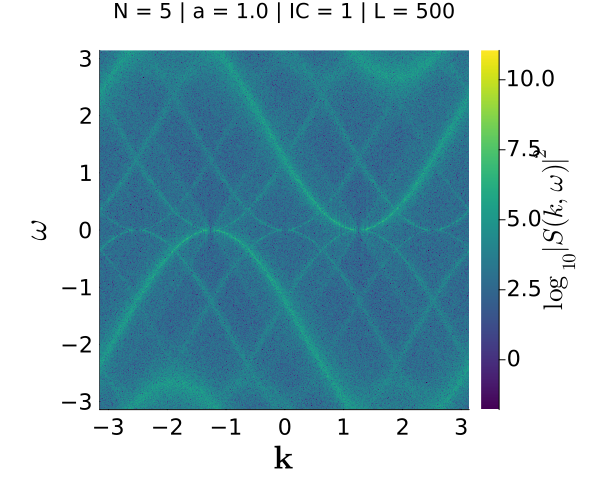
\includegraphics[width=\linewidth]{N5/a1p0_IC1_L500_trial1_komega.png}
    \caption{$k$--$\omega$ space}
  \end{subfigure}
  \caption{$N = 5$, $a = 1.0$, $L = 500$.}
\end{figure}

\clearpage
% =======================================================================
\section{$N = 6$ \quad ($L = 600$)}
% =======================================================================

\begin{figure}[H]
  \centering
  \begin{subfigure}{0.48\textwidth}
    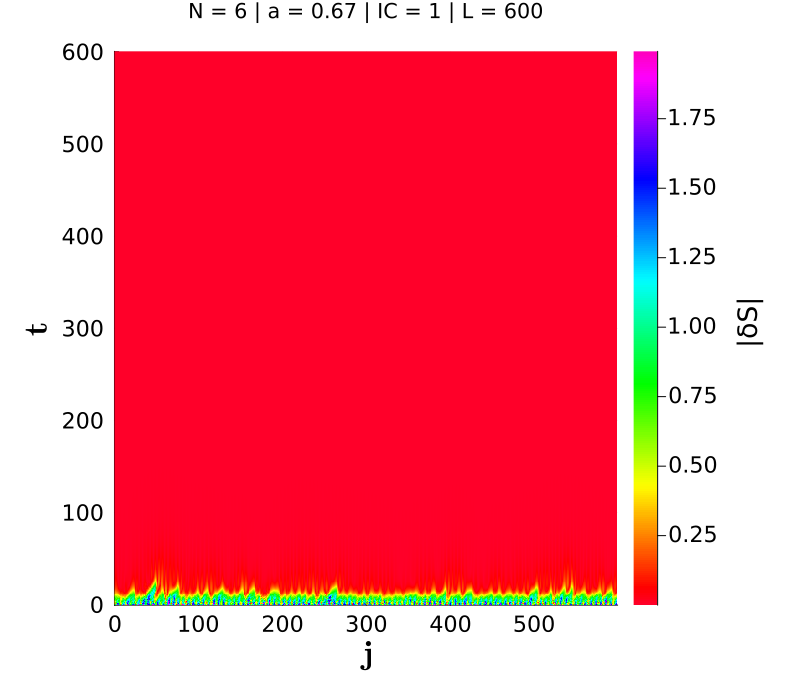
\includegraphics[width=\linewidth]{N6/a0p67_IC1_L600_trial1.png}
    \caption{Real space}
  \end{subfigure}\hfill
  \begin{subfigure}{0.48\textwidth}
    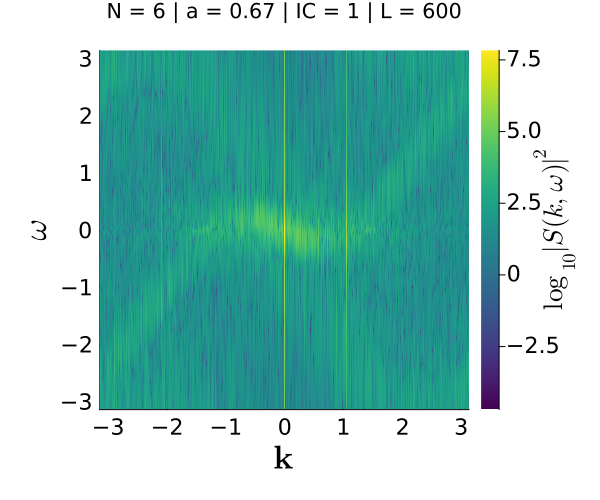
\includegraphics[width=\linewidth]{N6/a0p67_IC1_L600_trial1_komega.png}
    \caption{$k$--$\omega$ space}
  \end{subfigure}
  \caption{$N = 6$, $a = 0.67$, $L = 600$.}
\end{figure}

\begin{figure}[H]
  \centering
  \begin{subfigure}{0.48\textwidth}
    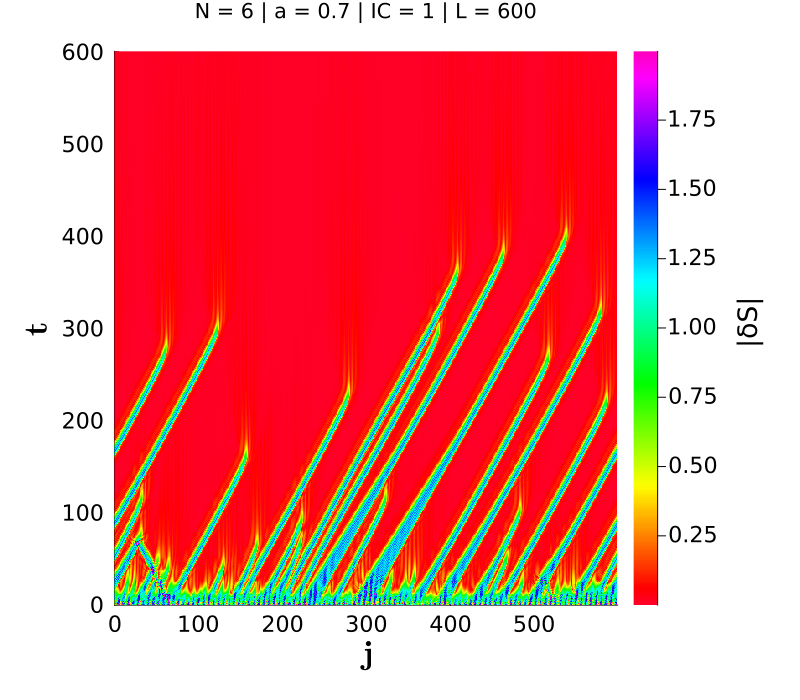
\includegraphics[width=\linewidth]{N6/a0p7_IC1_L600_trial1.png}
    \caption{Real space}
  \end{subfigure}\hfill
  \begin{subfigure}{0.48\textwidth}
    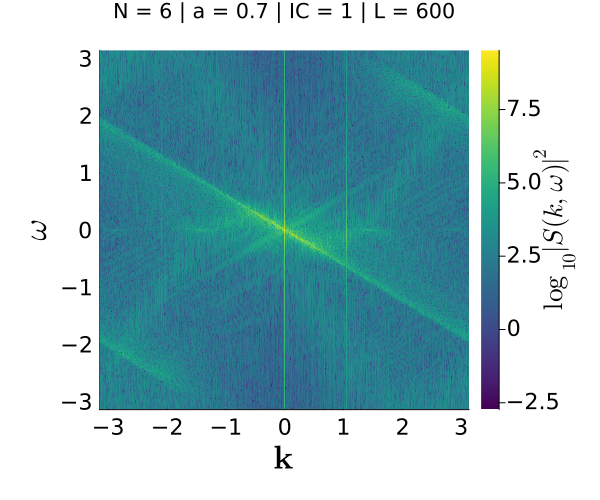
\includegraphics[width=\linewidth]{N6/a0p7_IC1_L600_trial1_komega.png}
    \caption{$k$--$\omega$ space}
  \end{subfigure}
  \caption{$N = 6$, $a = 0.7$, $L = 600$.}
\end{figure}

\begin{figure}[H]
  \centering
  \begin{subfigure}{0.48\textwidth}
    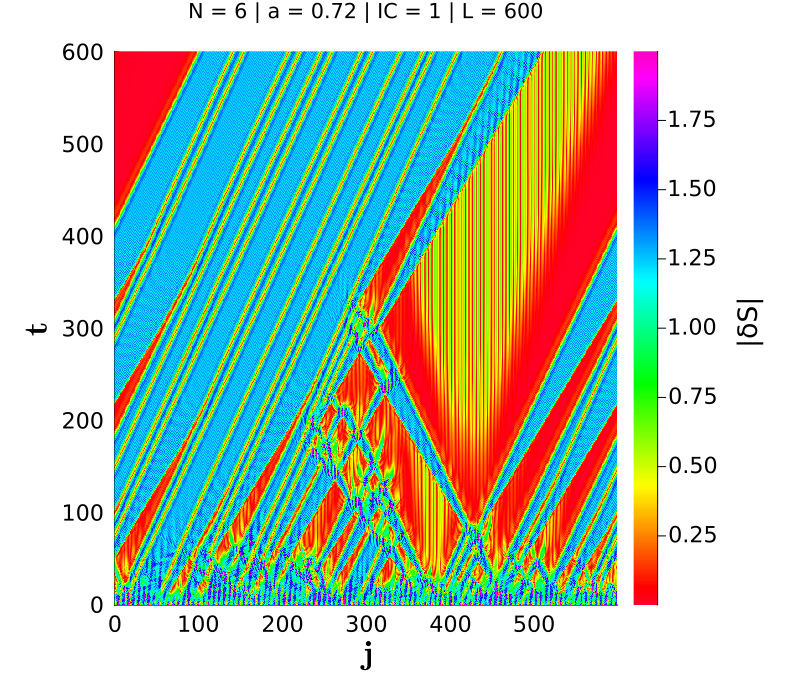
\includegraphics[width=\linewidth]{N6/a0p72_IC1_L600_trial1.png}
    \caption{Real space}
  \end{subfigure}\hfill
  \begin{subfigure}{0.48\textwidth}
    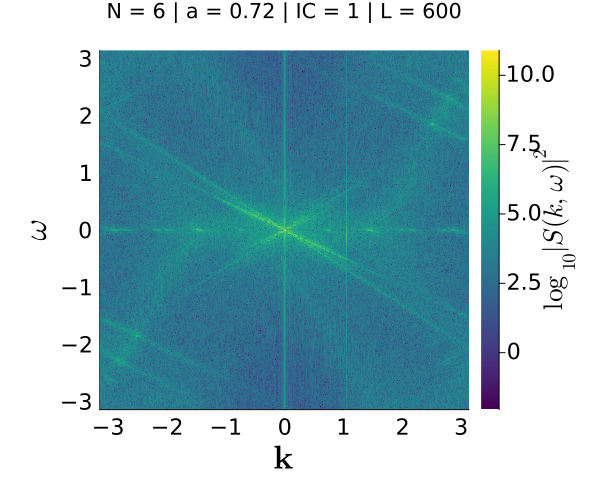
\includegraphics[width=\linewidth]{N6/a0p72_IC1_L600_trial1_komega.png}
    \caption{$k$--$\omega$ space}
  \end{subfigure}
  \caption{$N = 6$, $a = 0.72$, $L = 600$.}
\end{figure}

\begin{figure}[H]
  \centering
  \begin{subfigure}{0.48\textwidth}
    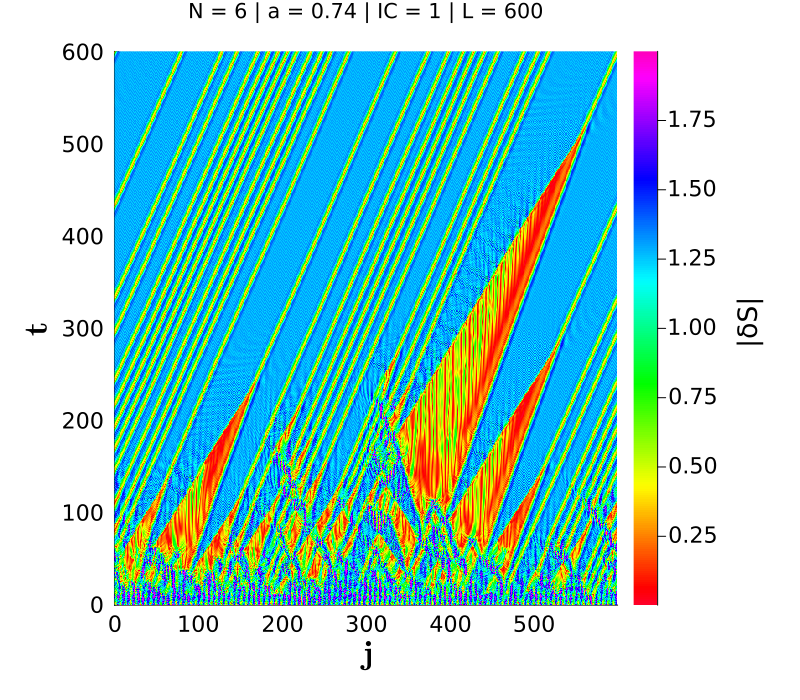
\includegraphics[width=\linewidth]{N6/a0p74_IC1_L600_trial1.png}
    \caption{Real space}
  \end{subfigure}\hfill
  \begin{subfigure}{0.48\textwidth}
    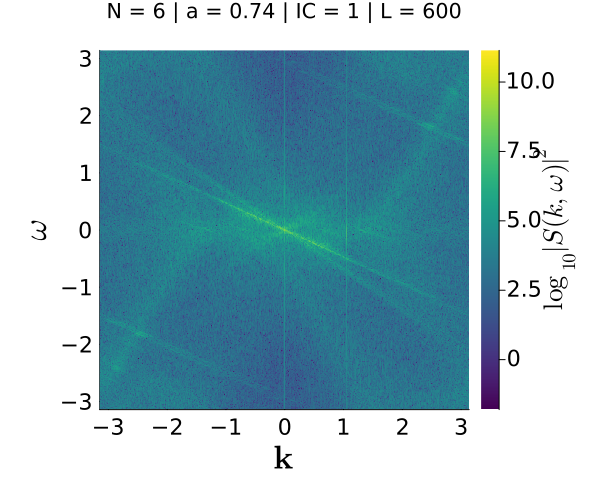
\includegraphics[width=\linewidth]{N6/a0p74_IC1_L600_trial1_komega.png}
    \caption{$k$--$\omega$ space}
  \end{subfigure}
  \caption{$N = 6$, $a = 0.74$, $L = 600$.}
\end{figure}

\begin{figure}[H]
  \centering
  \begin{subfigure}{0.48\textwidth}
    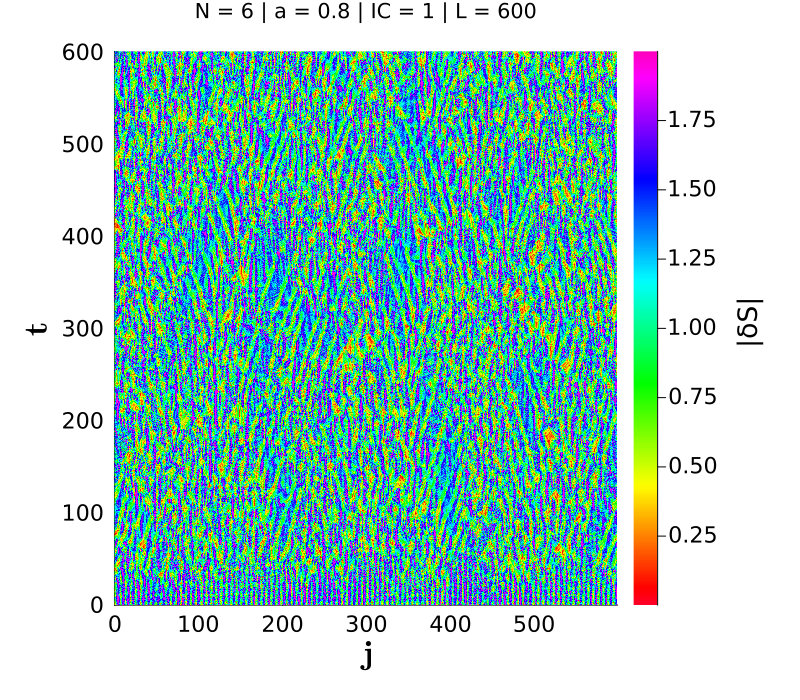
\includegraphics[width=\linewidth]{N6/a0p8_IC1_L600_trial1.png}
    \caption{Real space}
  \end{subfigure}\hfill
  \begin{subfigure}{0.48\textwidth}
    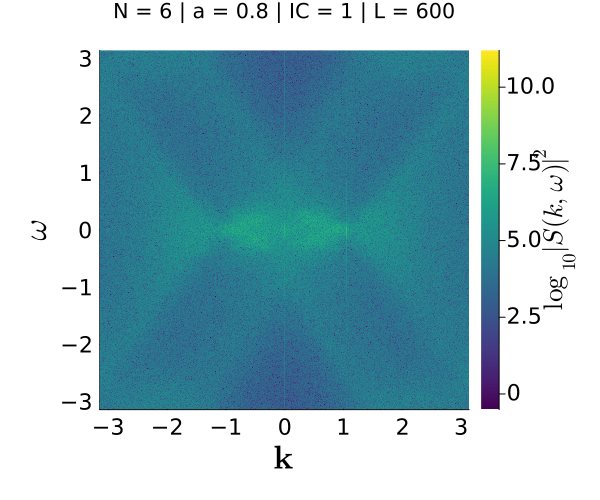
\includegraphics[width=\linewidth]{N6/a0p8_IC1_L600_trial1_komega.png}
    \caption{$k$--$\omega$ space}
  \end{subfigure}
  \caption{$N = 6$, $a = 0.8$, $L = 600$.}
\end{figure}

\begin{figure}[H]
  \centering
  \begin{subfigure}{0.48\textwidth}
    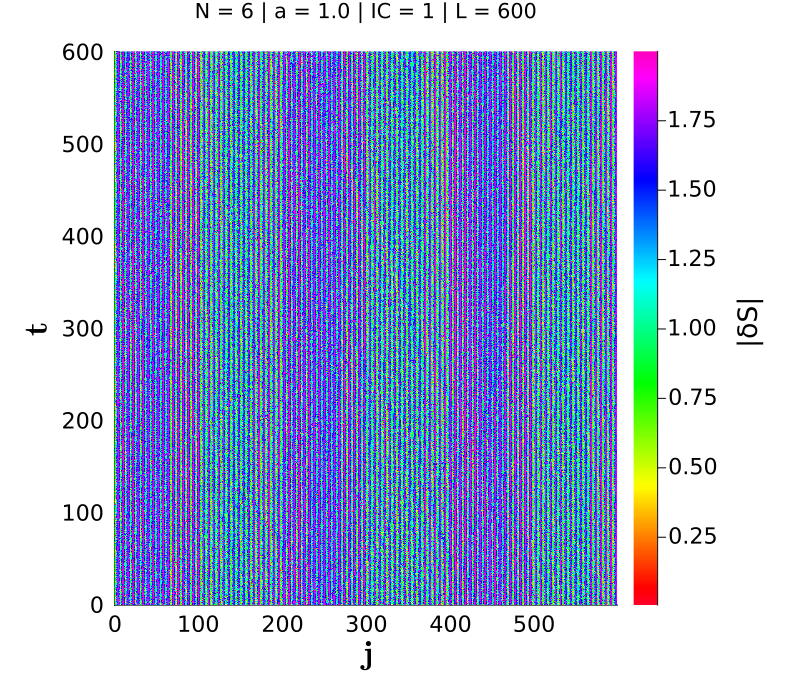
\includegraphics[width=\linewidth]{N6/a1p0_IC1_L600_trial1.png}
    \caption{Real space}
  \end{subfigure}\hfill
  \begin{subfigure}{0.48\textwidth}
    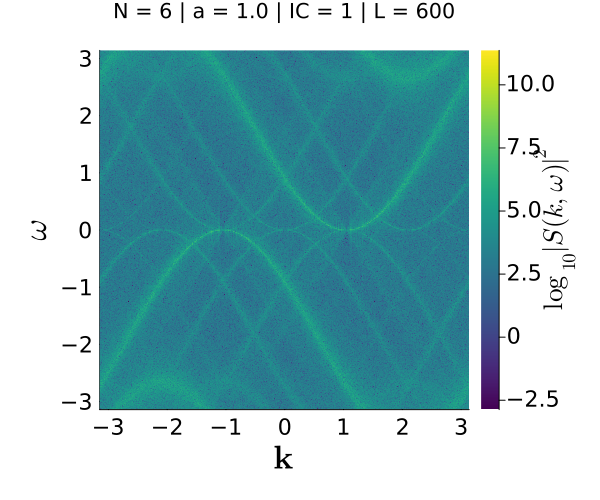
\includegraphics[width=\linewidth]{N6/a1p0_IC1_L600_trial1_komega.png}
    \caption{$k$--$\omega$ space}
  \end{subfigure}
  \caption{$N = 6$, $a = 1.0$, $L = 600$.}
\end{figure}

\end{document}
